%%% vers2.tex --- 

%% Author: xtroce@BhfMission.spuerwerk.net
%% Version: $Id: vers2.tex,v 0.0 2010/06/03 14:48:56 xtroce Exp$


\documentclass[12pt,draft,a4paper]{article}
\usepackage[debugshow,final]{graphicx}

%%\revision$Header: /home/xtroce/uni/2009-2010/2ejp/tjpstereovision/doc/vers2.tex,v 0.0 2010/06/03 14:48:56 xtroce Exp$

\graphicspath{{./images/}}

\begin{document}

\section{Dense stereo}
\subsection{Theory}
Dense stereo combines the two images you get from the rectification
and calculates the position of the pixels in the left images and
outputs where the pixel sits in the right  image. With this method you
can calcluate the distance from the pixel from the center point of
view. The depth is then translated in a depth picture where close
points are almost white and points further away are almost
black. Points inbetween are shown on a grayscale, which gets darker
 the further the point is away from the camera.\\

\begin{figure}
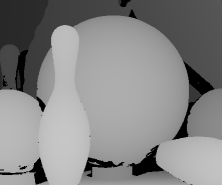
\includegraphics[width=8cm]{depthmap}
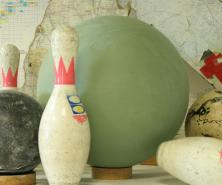
\includegraphics[width=8cm]{depthmap_original}
\end{figure}

To archieve this you have a whole list of algorithms which could do
the trick. A good overview can be found at: \\
http://vision.middlebury.edu/stereo/eval/ \\
Most of these algorithms are based on 4 principles: 

\begin{itemize}
\item Graph Cut
\item Believe Propagation
\item Region Based
\item Dynamic Programming
\end{itemize}

These algorithms have to deal with following different problems in their
calculations.

\begin{itemize}
    \item Matching points in both images
    \item Occlusion
\end{itemize}

\subsubsection{Matching}
The main goal of such an algorithm is the possibility of matching one
point in one image with the same point in the other image. During the
matching there are several tasks that the algothim has to overcome. At
first it has to compare the epibolar lines of the images pixel by
pixel. For every pixel on one line you have to find the counterpart on
the other line. Often the pixels aren't in the same order, if
i.e. there is a lamp pole in front of a house, things that lie on
the left side of the lamp pole in the left picture sit on the right
side on the right picture.

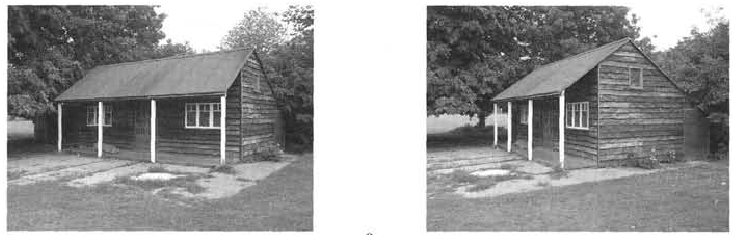
\includegraphics{matching_problems_direction}  

Another problem is occlusion of the pixels. Some things that are
visible in one picture are hidden behind objects in the other
picture. This has to be caught and handled.

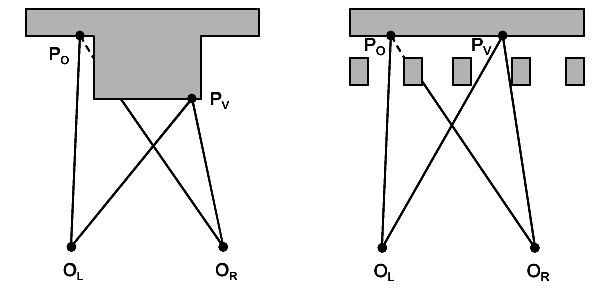
\includegraphics{matching_problems_occlusion}

Because the openCV library that we have chosen has the basic
implementation of a graph cut algorithm from Kolmogorov. It is a bit
slow and not the best algorithm to handle occlusion but because it is
easy to use we will at first use this algorithm and later replace it
with a better working version.


%%%%##########################################################################

\end{document}
